\documentclass[14pt]{beamer}
%\documentclass[handout]{beamer} %Makes Handouts
\usetheme{Singapore} %Gray with fade at top
\useoutertheme[subsection=false]{miniframes} %Supppress subsection in header
\useinnertheme{rectangles} %Itemize/Enumerate boxes
\usecolortheme{seagull} %Color theme
\usecolortheme{rose} %Inner color theme

\definecolor{light-gray}{gray}{0.75}
\definecolor{dark-gray}{gray}{0.55}
\setbeamercolor{item}{fg=light-gray}
\setbeamercolor{enumerate item}{fg=dark-gray}

\setbeamertemplate{navigation symbols}{}
%\setbeamertemplate{mini frames}[default]
%\setbeamercovered{dynamics}
\setbeamerfont*{title}{size=\Large,series=\bfseries}

%\setbeameroption{notes on second screen} %Dual-Screen Notes
%\setbeameroption{show only notes} %Notes Output

\setbeamertemplate{frametitle}{\vspace{.5em}\bfseries\insertframetitle}
\newcommand{\heading}[1]{\noindent \textbf{#1}\\ \vspace{1em}}

% small footnotes
\setbeamerfont{footnote}{size=\tiny}

\usepackage{bbding,color,multirow,times,ccaption,tabularx,graphicx,booktabs}
\usepackage{colortbl} %Table overlays
\usepackage[english]{babel}
\usepackage[latin1]{inputenc}
\usepackage[T1]{fontenc}
\usepackage{lmodern}
\usepackage{alltt}

\author[]{Thomas J. Leeper}
\institute[]{
  \inst{}%
  Department of Government\\London School of Economics and Political Science
}

\usepackage{tikz}
\usetikzlibrary{shapes,arrows}
\usepackage[normalem]{ulem}

\title{What role can surveys play in behavioural science?}

\date[]{18 January 2018\\LSE Executive MSc Behavioural Science}

\begin{document}

\frame{\titlepage}

\frame{
\frametitle{About Me}

\begin{itemize}\itemsep1em
\item Associate Professor at LSE
\item PhD from Northwestern University (2012)
\item Research interests
	\begin{itemize}
	\item Political psychology
	\item Survey--experimental methods
	\item Reproducible computational social science
	\end{itemize}
\end{itemize}
}


\frame{}


\frame{

\frametitle{Premise}

\begin{itemize}\itemsep1em
\item<2-> A survey is any questionnaire-based method of data collection in which most data is produced through ``self-reports''
\item<3-> Surveys are obviously useful for studying \textit{characteristics}, \textit{beliefs}, and \textit{attitudes}
\item<4-> Surveys are not often seen as useful for studying \textit{behaviour}
\end{itemize}

}


\frame{
\frametitle{Goals for today}

By the end of today you should be able to:

\begin{enumerate}\itemsep1em
\item Describe the relationship between (and distinction between) attitudes and behaviours
\item Identify the limitations of survey measures of past behaviours and behavioural intentions
\item Evaluate possible strategies for improving behavioural self-reporting
\item Apply direct, survey-based measures of behaviour to your own work
\end{enumerate}
}

\frame{}
\frame{\tableofcontents}



\section{Attitudes vs. Behaviours}
\frame{\tableofcontents[currentsection]}

\frame{
\frametitle{Definitions}
\begin{itemize}\itemsep2em
\item Attitude: ``a psychological tendency that is expressed by evaluating a particular entity with some degree of favour or disfavour'' \footnote{Eagly and Chaiken, 1998, ``Attitude Structure and Function.'' \textit{Handbook of Social Psychology}, p.269.}
\item Behavior: ``The actions by which an organism adjusts to its environment.'' (APA)
\end{itemize}
}

\frame{
\large
\begin{center}
\only<2->{How many of you feel that it is important for citizens to vote?}

\vspace{2em}

\only<3->{How many of you voted in the \textit{most recent local election} in which you were eligible to cast a ballot?}
\end{center}
}


\frame{
\large
\begin{center}
What are some behaviours that practising behavioural scientists might care about? (Think about any domain or context.)
\end{center}
}



\frame{
\frametitle{Why should behavioural scientists care about attitudes?}
\begin{itemize}\itemsep1em
\item<2-> Care about attitudes per se, e.g.:
	\begin{itemize}
	\item<3-> To represent public opinions in policymaking
	\item<3-> To assess sentiment or satisfaction
	\item<3-> To try to change those views
	\end{itemize}
\item<4-> Care about attitudes because they induce \textit{behaviour}
\item<5-> Attitudes are relatively easy to measure on questionnaire/survey methods but behaviours not so much
\end{itemize}
}

\frame<1-2>[label=theories]{

\frametitle{From attitudes to behaviours?}

Early psychology research showed limited connection between attitudes and associated behaviours\\

\begin{itemize}\itemsep1em
\item<2-> \textit{Theory of Planned Behavior} (Ajzen)
	\begin{itemize}
	\item From \textit{Theory of Reasoned Action} (Ajzen \& Fishbein)
	\item Attitudes interact with both subjective norms and ``perceived behavioural control''
	\end{itemize}
\item<3-> Other traditions
	\begin{itemize}
	\item \textit{MODE} (Fazio), a ``dual process'' framework
	\item \textit{Health Belief Model}
	\item Theories of habit
	\item Cost-benefit analysis
	\end{itemize}
\end{itemize}

}


\frame{
\begin{center}
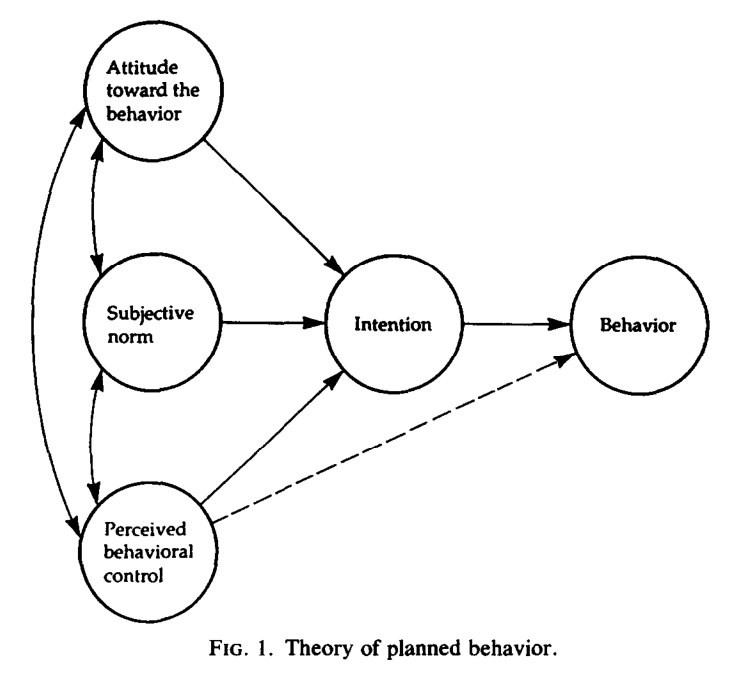
\includegraphics[height=.9\textheight]{images/Ajzen1991-Figure1.png}
\end{center}

\vspace{1em}

{\footnotesize Ajzen (1991). ``The Theory of Planned Behaviour.'' \textit{Org B \& Hum. Dec. Proc.} 50: 179--211}
}

\againframe<2->{theories}



\frame{

\frametitle{From attitudes to behaviours?}

\begin{itemize}\itemsep1em
\item Basically, there are many reasons why attitudes do not correlate very highly with behaviours

\item People may also have attitudes toward the behaviours themselves (e.g., wanting to act on attitude but disfavouring a given action)

\item Attitude strength is possibly critical (but conceptually murky)
\end{itemize}

}

\frame{

\frametitle{\normalsize{Behaviour Change without Attitude Change}}

\begin{itemize}\itemsep1em
\item Recent behavioural science research suggests some behaviours can change dramatically without changing attitudes

	\begin{itemize}
	\item Nudges related to charitable donations
	\item Increasing vaccination even as attitudes toward vaccination become more negative
	\end{itemize}

\item If we want to study \textit{behaviour} per se, maybe we don't need to know much about attitudes!
\end{itemize}

}


% Wicker (1969)
% Ajzen and Fishbein (1977)
% Ajzen 
% Fazio (1986) book: "How do attitudes guide behavior?"
% Fazio and Towles-Schwen (1999)
% Armitage and Conner (2001)


\frame{}


\section[Measurement Problems]{Problems with Behavioural Self-Reports}
\frame{\tableofcontents[currentsection]}


\frame{
\frametitle{Some Common Wisdom}
\large
\begin{center}
Surveys are a good instrument for measuring and studying attitudes!

\vspace{1em}

\only<2->{But attitudes are not the same as behaviours!}

\vspace{1em}

\only<3->{Therefore, surveys are a poor instrument for measuring and studying behaviours!}

\end{center}
}

\frame{
\frametitle{Concern 1:\\Self-reports are not behaviours}
\begin{itemize}\itemsep1em
\item A survey questionnaire measures ``responses'' expressed in words, numbers, and other trivial actions
\item These are obviously not behaviours but reports of behaviours.
\item<2-> Questionnaires can, however, measure \textit{behavioural intentions} and \textit{self-reported past behaviour}
\end{itemize}
}


\frame{
\frametitle{Concern 2:\\Behavioural intentions are poor predictors of behaviour}
\begin{itemize}\itemsep0.5em
\item All three models of attitude--behaviour linkage suggest the effect of attitudes on behaviours is conditional
	\begin{itemize}
	\item TRA: Depends on subjective norms
	\item TPB: Also depends on behavioural control
	\item MODE: Also depends on motivation and opportunity
	\end{itemize}
\item<2-> Behavioural intention questions do not effectively measure future behaviour
\item<3-> Questionnaires can measure \textit{past behaviour}
\end{itemize}
}


\frame{
\frametitle{Concern 3:\\Survey measures of past behaviour lack validity}
\begin{itemize}\itemsep1em
\item<2-> Many different, imperfect operationalizations:
	\begin{itemize}
	\item ``Have you ever\dots?''
	\item ``When was the last time\dots?''
	\item ``How many times in the past <PERIOD> have you\dots?''
	\item ``How many <TIME UNIT> in the past <PERIOD> have you spent\dots?''
	\end{itemize}
\item<3-> Numerous issues emerge here!
\end{itemize}
}


\frame{

\frametitle{Problems with self-reports}

Rarely correspond to direct ``true'' measures behaviour. Why?

\begin{itemize}\itemsep0.5em
\item<2-> Recall failure and false memories
\item<3-> Reference period ambiguity and lags
\item<4-> Recency and primacy biases
\item<5-> Social desirability biases
\item<6-> Construct invalidity
\end{itemize}

}

\frame{
\frametitle{Example: Prior (2009)\footnote{Prior. 2009. ``Improving Media Effects Research through Better Measurement of News Exposure.'' \textit{Journal of Politics} 71(3): 893--908. \href{http://doi.org/10.1017/S0022381609090781}{doi:10.1017/S0022381609090781}}}
\only<1>{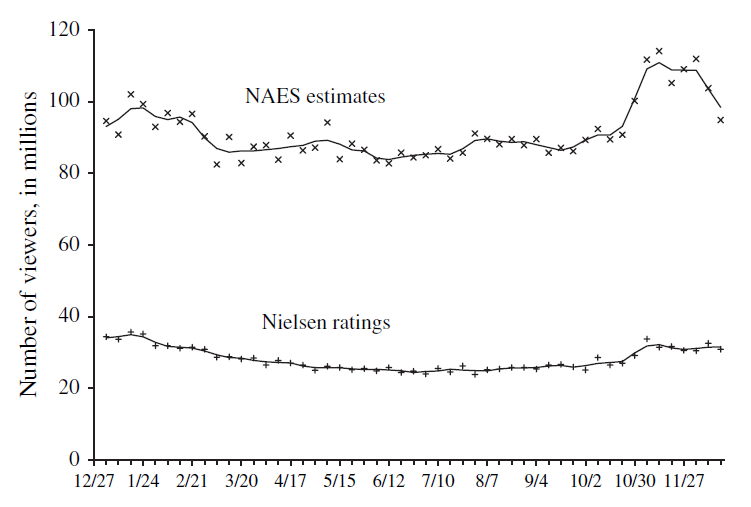
\includegraphics[height=.7\textheight]{images/prior.png}}
\only<2->{
	\begin{itemize}\itemsep0.5em
	\item<2-> Prior argues that recall of hours television watched and specific programmes watched is too cognitively challenging
	\item<3-> Suggests using population benchmarks to provide ``anchoring''
	\end{itemize}
}
}



\frame{

\frametitle{Example:\\Holbrook \& Krosnick (2016)\footnote{Holbrook \& Krosnick. 2013. ``A New Question Sequence to Measure Voter Turnout in Telephone Surveys.'' \textit{Public Opinion Quarterly} 77: 106--23. \href{http://doi.org/10.1093/poq/nfs061}{doi:10.1093/poq/nfs061}}}

\begin{itemize}\itemsep0.5em
\item<1-> People massively overreport voting in elections
\item<2-> Past experiments show that giving respondents excuses for why others may not have voted lower reported turnout but not fully
\item<3-> Their design does two things:
	\begin{itemize}
	\item Measures self-reported past intention
	\item Primes respondents with those excuses and asks for how those excuses might have led them to deviate from their intentions
	\end{itemize}
\end{itemize}

}



\frame{

\frametitle{Some provisional conclusions}

\begin{enumerate}\itemsep1em
\item It is hard to write construct valid measures of past behaviour
\item Behavioural intentions are poorly predictive of future behaviour
\item So, behavioural self-reports are very problematic!
\item<2-> Thesis: focus on behaviours that can be measured within a survey context!
\end{enumerate}

}

\frame{
\large
\begin{center}
\textbf{Abandon behavioural self-reports?}
\vspace{2em}

\only<2->{Sometimes we have no choice but to rely on a self-reported measure of past behaviour or future behavioural intentions!}
\end{center}
}

\frame{
\frametitle{Improving Self-Reports}
\begin{itemize}
\item<2-> Use unambiguous, short, and recent reference periods
\item<3-> Provide population benchmarks
\item<4-> Excuse socially undesirable behaviour
\item<5-> Use alternative survey modes to avoid social desirability
\item<6-> Try probabilistic measures of intention\footnote{Delavande and Manski. 2010. ``Probabilistic Polling and Voting in the 2008 Presidential Election.'' \textit{Public Opinion Quarterly} 74(3): 433--59.}
\item<7-> Validate self-reports against actual behaviour where possible
\end{itemize}
}

% (e.g., live data capture; location data; web-tracking; etc.) - usefully applied by Google Surveys

\section[Behavioural Measures]{Credible Behavioural Measures in Surveys}
\frame{\tableofcontents[currentsection]}


\frame{
\frametitle{Behavioural measures}
All hope is not lost! There are some behaviours that can be directly measured through survey questionnaires.

\vspace{1em}

\only<2->{Three broad categories:}
\begin{enumerate}
\item<3-> Behavioural measures that provide survey paradata % (response latency, reading times, answer switching, nonresponse)
\item<4-> Behavioural measures that operationalize attitudes % IAT
\item<5-> Behavioural measures that operationalize behaviours % (e.g., political participation; purchasing)
\end{enumerate}
}


\frame{
\frametitle{Behavioural Measures for Paradata}

Why?
	\begin{itemize}
	\item Respondents use of the survey tells us something meaningful about their behaviour
	\end{itemize}

\vspace{1em}
\only<2->{What?
	\begin{itemize}
	\item<3-> Nonresponse
	\item<4-> Response latencies
	\item<5-> Reading times
	\item<6-> Answer switching
	\item<7-> Eye tracking
	\item<8-> Mouse tracking
	\item<9-> Smartphone metadata
	\end{itemize}
}
}


\frame{
\frametitle{Behavioural Measures for Attitudes}

Why?
	\begin{itemize}
	\item Attitudinal self-reports might be ``cheap talk''
	\end{itemize}

\vspace{1em}
\only<2->{What?
	\begin{itemize}
	\item<3-> Implicit Association Test
	\item<4-> Incentivized Survey questions
	\end{itemize}
}
}


\frame{

\frametitle{Implicit Association Test}

\large
\url{https://implicit.harvard.edu/}

}


\frame{
\begin{center}
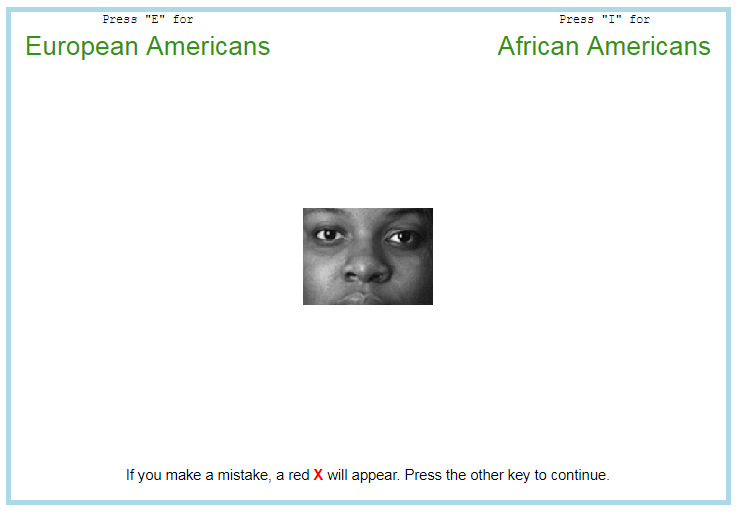
\includegraphics[width=\textwidth]{images/implicit1.png}
\end{center}
}

\frame{
\begin{center}
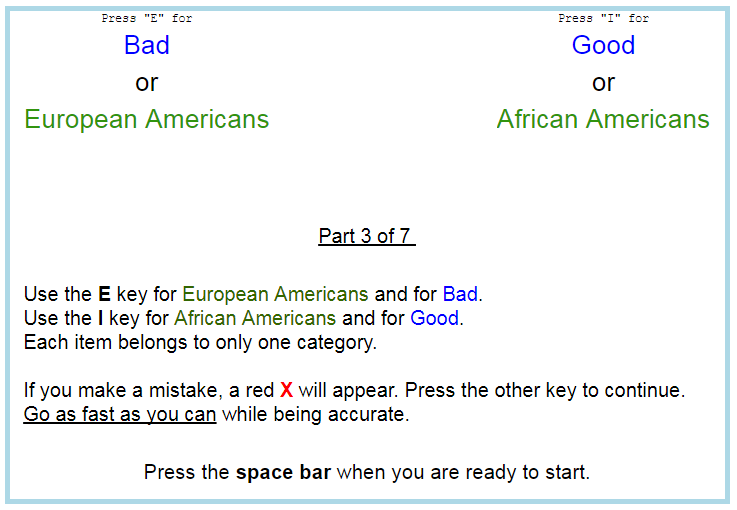
\includegraphics[width=\textwidth]{images/implicit2.png}
\end{center}
}

\frame{
\begin{center}
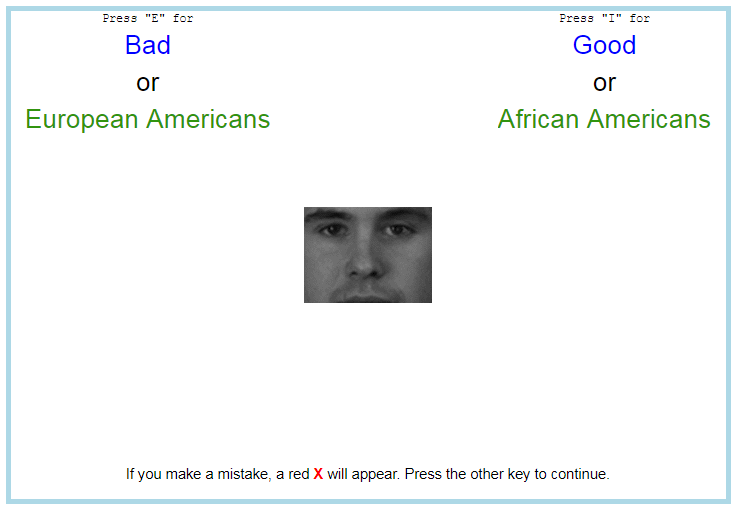
\includegraphics[width=\textwidth]{images/implicit3.png}
\end{center}
}


\frame<1>[label=incentivised]{
\frametitle{Example 3:\\Incentivised Survey Questions}

Definitions:

\begin{itemize}\itemsep0.5em
\item A survey question is just a self-report
\item An \textit{incentivized} survey question attached financial gains or losses to the answer options
\end{itemize}

\vspace{1em}
\only<2->{
Paradigm could be applied to any measure of behavioural intentions to avoid cheap talk.
}

}

\frame{

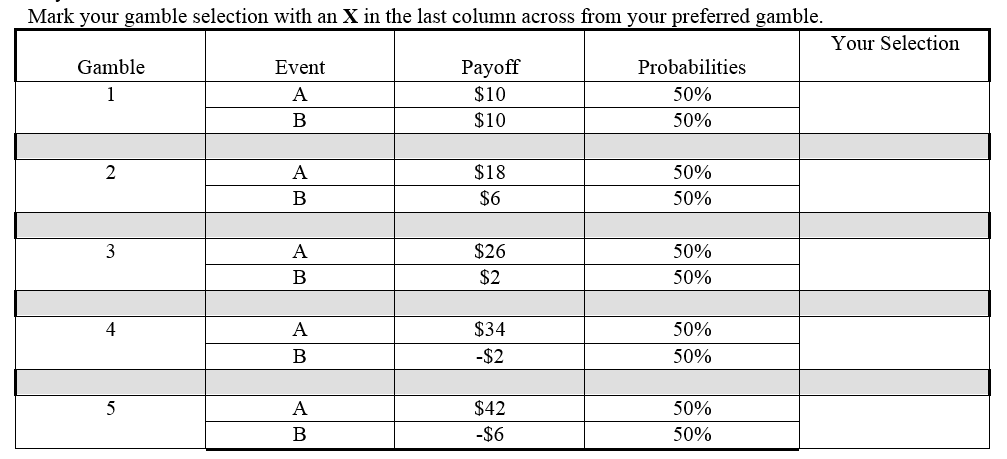
\includegraphics[width=\textwidth]{images/eckelgrossman.png}

\vspace{2em}
{\tiny Eckel \& Grossman. 2008 ``Forecasting risk attitudes.'' \textit{Journal of Economic Behavior \& Organization} 68(1): 1--17. \href{http://doi.org/10.1016/j.jebo.2008.04.006}{doi:10.1016/j.jebo.2008.04.006}\par }
}

\againframe<1->{incentivised}



\frame{

\frametitle{Behavioural Measures for Behaviour}

Why?
	\begin{itemize}
	\item We want to observe or affect behaviour (e.g., in an experiment)
	\end{itemize}
	
\vspace{1em}
\only<2->{What? 
	\begin{itemize}
	\item Directly measure or initiate a direct measure of a behaviour
	\item May be measured by something that occurs within the confines of the survey or something outside of the survey
	\end{itemize}
}
}


\frame<1-2>[label=infochoice]{

\frametitle{Example 1:\\Active Information Choice}

\begin{itemize}\itemsep0.5em
\item<2-> ``Followed link'' identification\footnote{Guess, AM. 2015. ``Measure for Measure.'' \textit{Political Analysis} 23: 59--75. \href{http://doi.org/10.1093/pan/mpu010}{doi:10.1093/pan/mpu010} }

\item<3-> Information boards\footnote{Leeper, TJ. 2014. ``The Informational Basis for Mass Polarization.'' \textit{Public Opinion Quarterly} 78(1): 27--46. \href{http://doi.org/10.1093/poq/nft045}{doi:10.1093/poq/nft045}}

\item<4-> Video choice\footnote{Arceneaux, K \& Johnson, M. 2012. \textit{Changing Minds or Changign Channels}. Chicago: The University of Chicago Press.}

\item<5-> Dynamic Process Tracing Environment \footnote{\url{https://dpte.polisci.uiowa.edu/dpte/}}
\end{itemize}

}

\frame{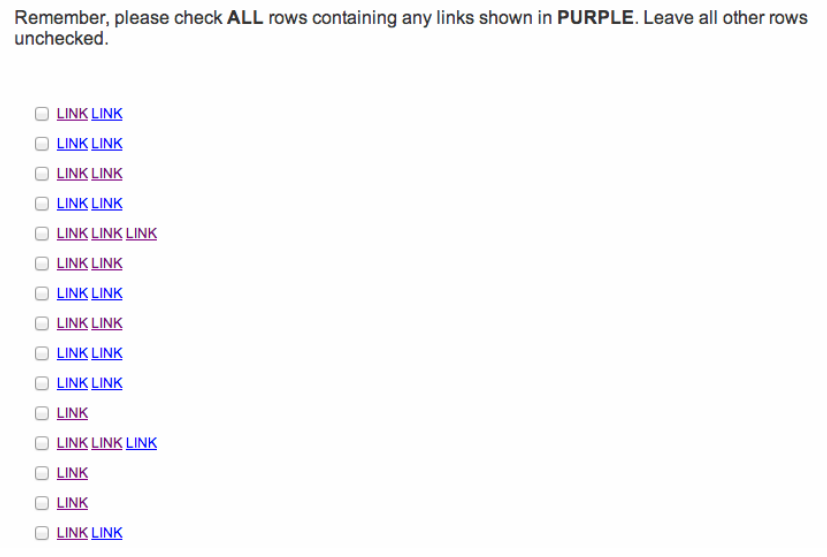
\includegraphics[width=\textwidth]{images/linksguess.png}}

\againframe<2-3>{infochoice}

\frame{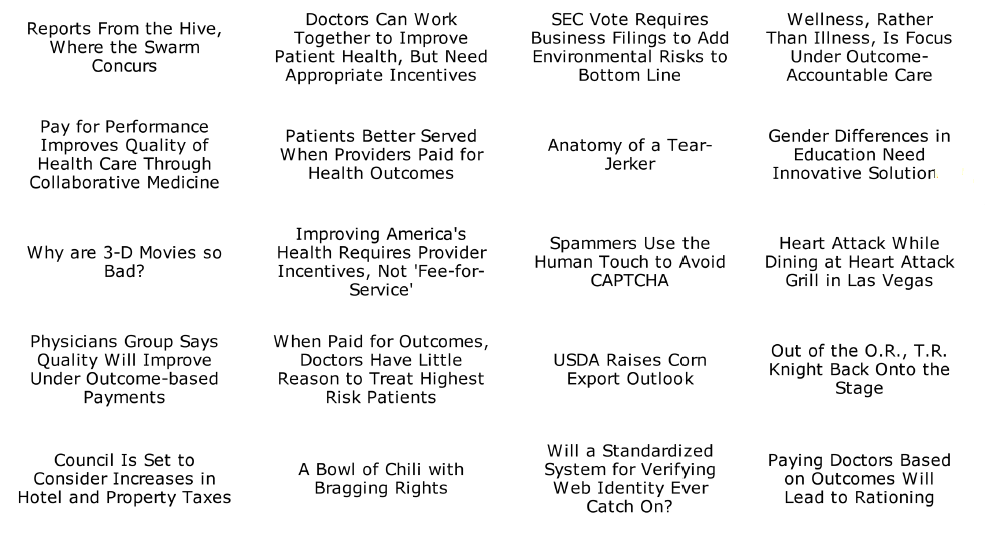
\includegraphics[width=\textwidth]{images/leeper.png}}

\againframe<3-5>{infochoice}

\frame{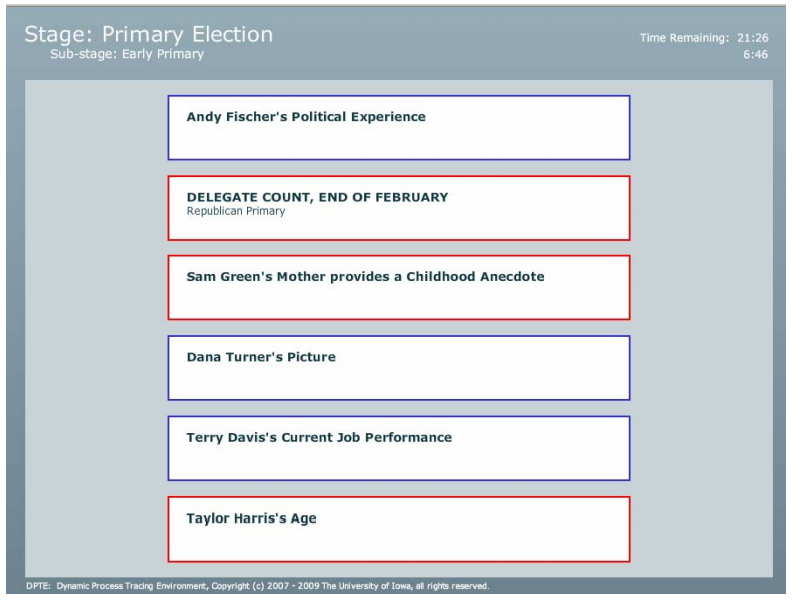
\includegraphics[width=\textwidth]{images/dpte1.png}}
\frame{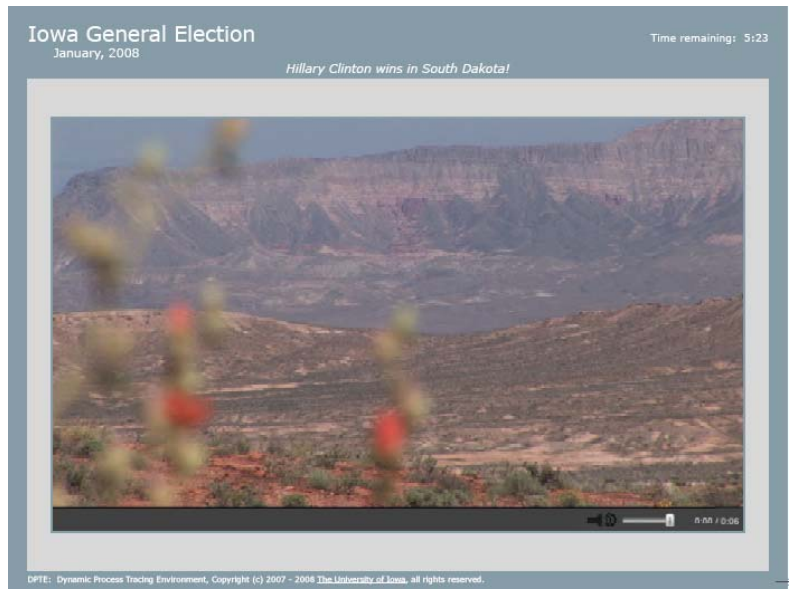
\includegraphics[width=\textwidth]{images/dpte2.png}}
\frame{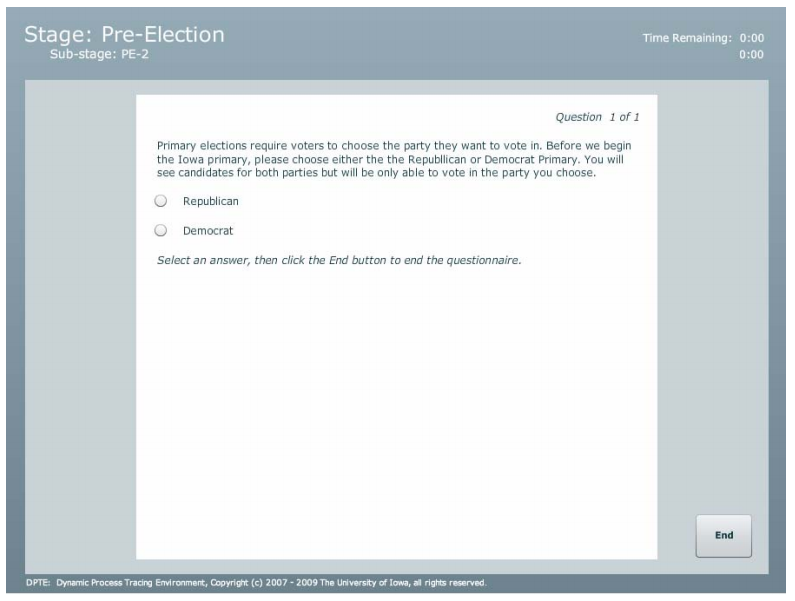
\includegraphics[width=\textwidth]{images/dpte3.png}}



\frame{

\frametitle{Example 2:\\Sign-up/Enrolment}

An extension of information choice behaviour would be explicit engagement in other kinds of (small) behaviours, such as:

\begin{itemize}\itemsep0.5em
\item Entering an email address to receive information or join a mailing list \footnote{Leeper, TJ. 2017. ``How Does Treatment Self-Selection Affect Inferences About Political Communication?'' \textit{Journal of Experimental Political Science}: In press.} \footnote{Bolsen, Druckman, \& Cook. 2014. ``Communication and Collective Actions.'' \textit{Journal of Experimental Political Science} 1(1): 24--38. \href{http://doi.org/10.1017/xps.2014.2}{doi:10.1017/xps.2014.2}}

\item Signing up for an appointment or further interaction
\end{itemize}

}

\frame<1-4>[label=purchasing]{
\frametitle{Example 3:\\Purchasing Decisions}

Common ways to study purchasing behaviour include:

\begin{itemize}
\item<2-> Direct attitudinal questions
\item<3-> Retrospective and prospective self-reports
\item<4-> Conjoint experiments
\end{itemize}

\only<5->{Another way is embedding a purchase in a survey.\footnote{Bolsen, T. 2011. ``A Lightbulb Goes On.'' \textit{Political Behavior} 35(1): 1--20.  \href{http://doi.org/10.1007/s11109-011-9186-5}{10.1007/s11109-011-9186-5}
}}

}

\frame{
\begin{center}
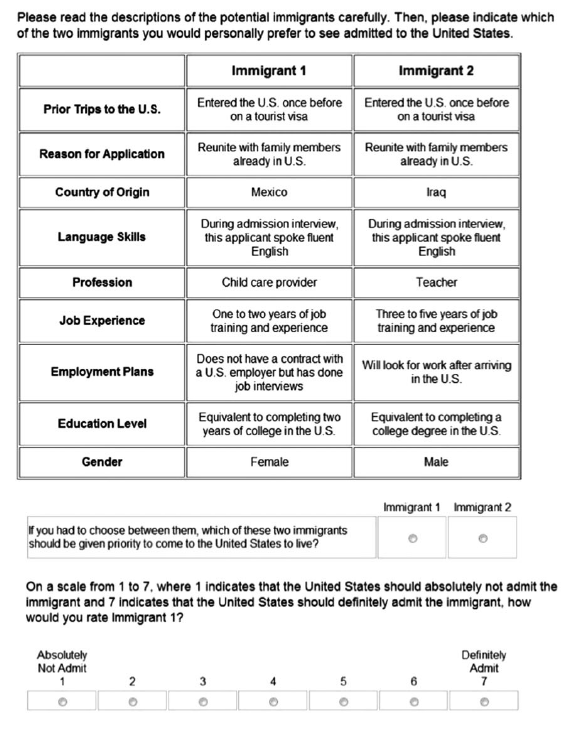
\includegraphics[height=\textheight]{images/hainmuelleretal.png}
\end{center}
}

\frame{
\begin{center}
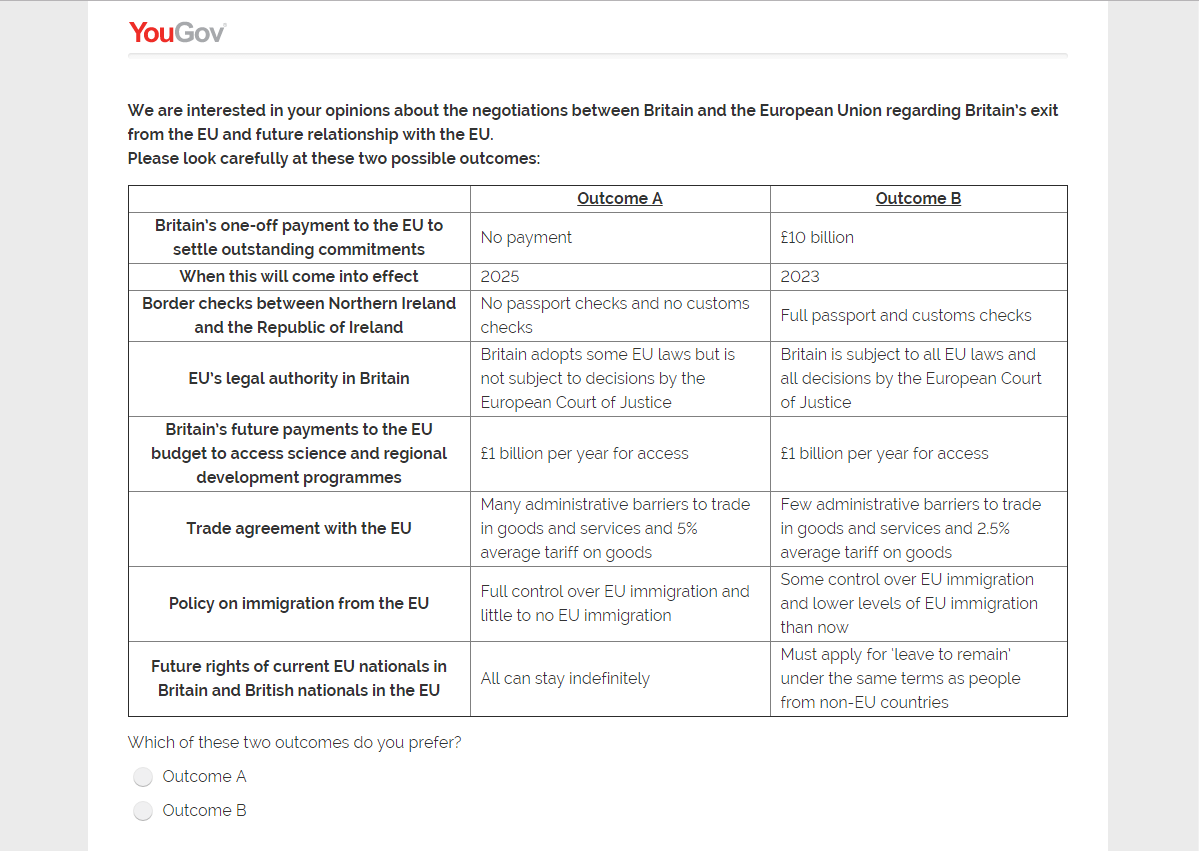
\includegraphics[width=\textwidth]{images/brexit-conjoint.png}
\end{center}
}


\againframe<4-5>{purchasing}

\frame{

\begin{center}
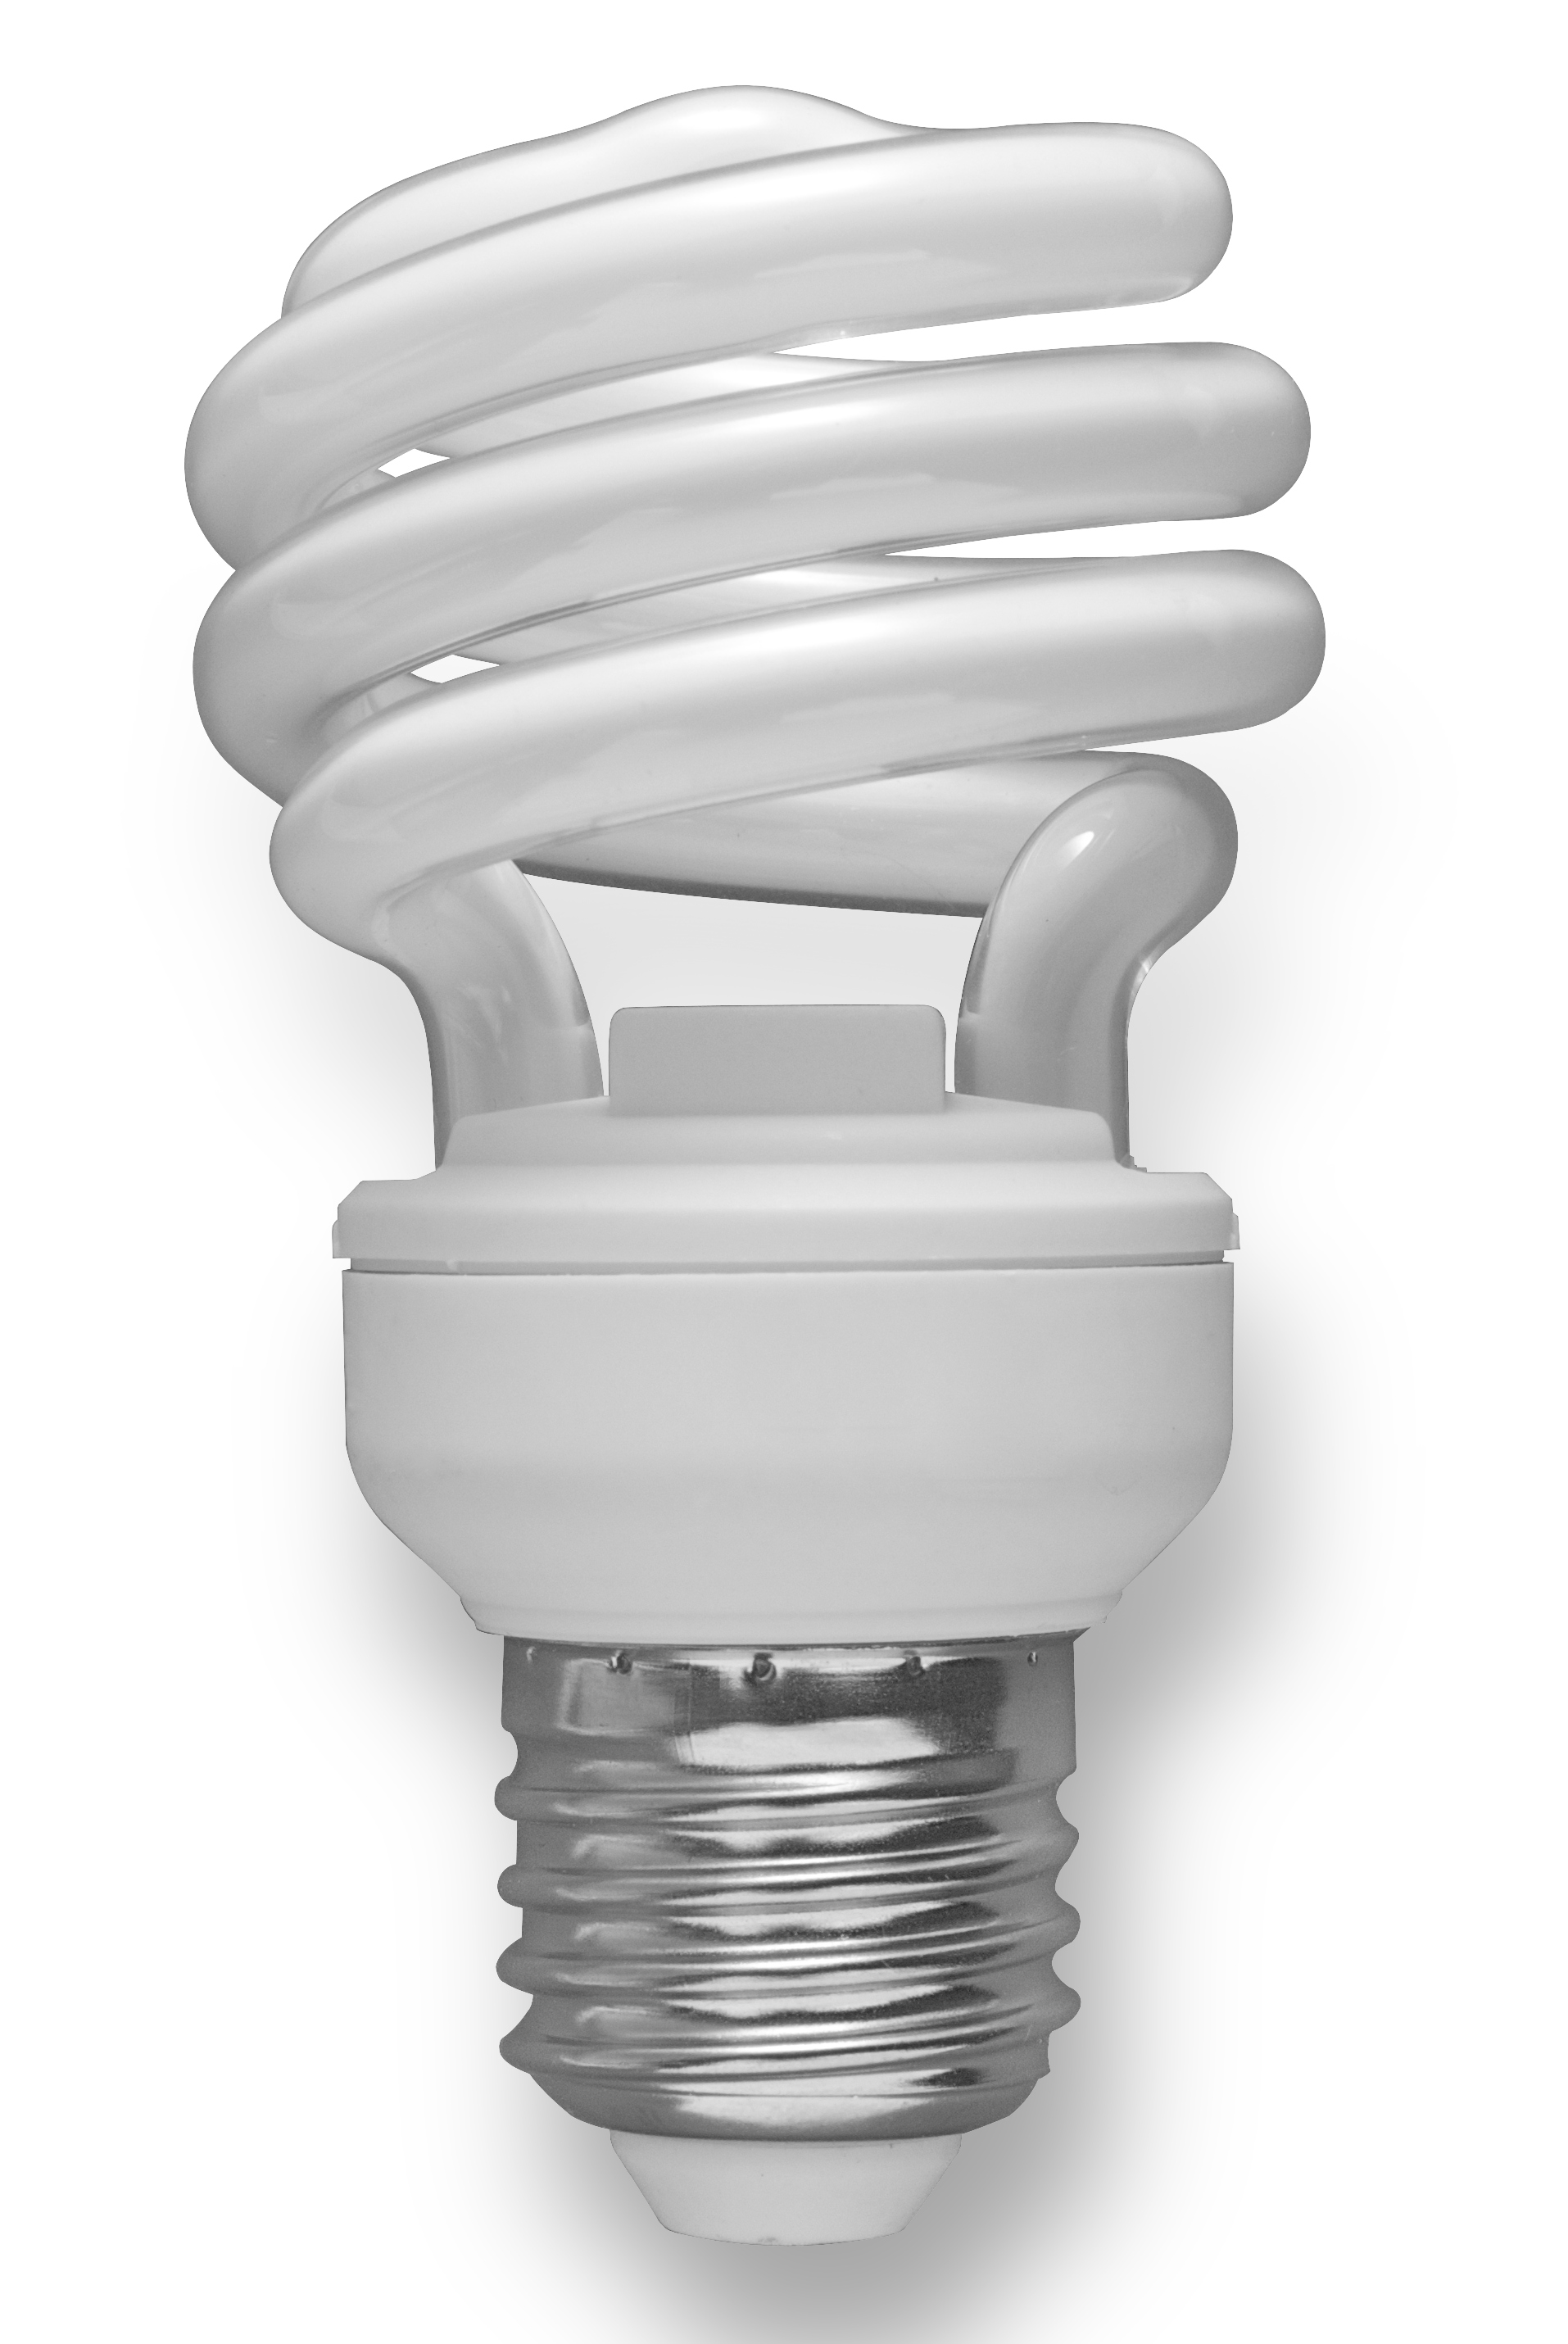
\includegraphics[width=.45\textwidth]{images/lightbulb1.png}
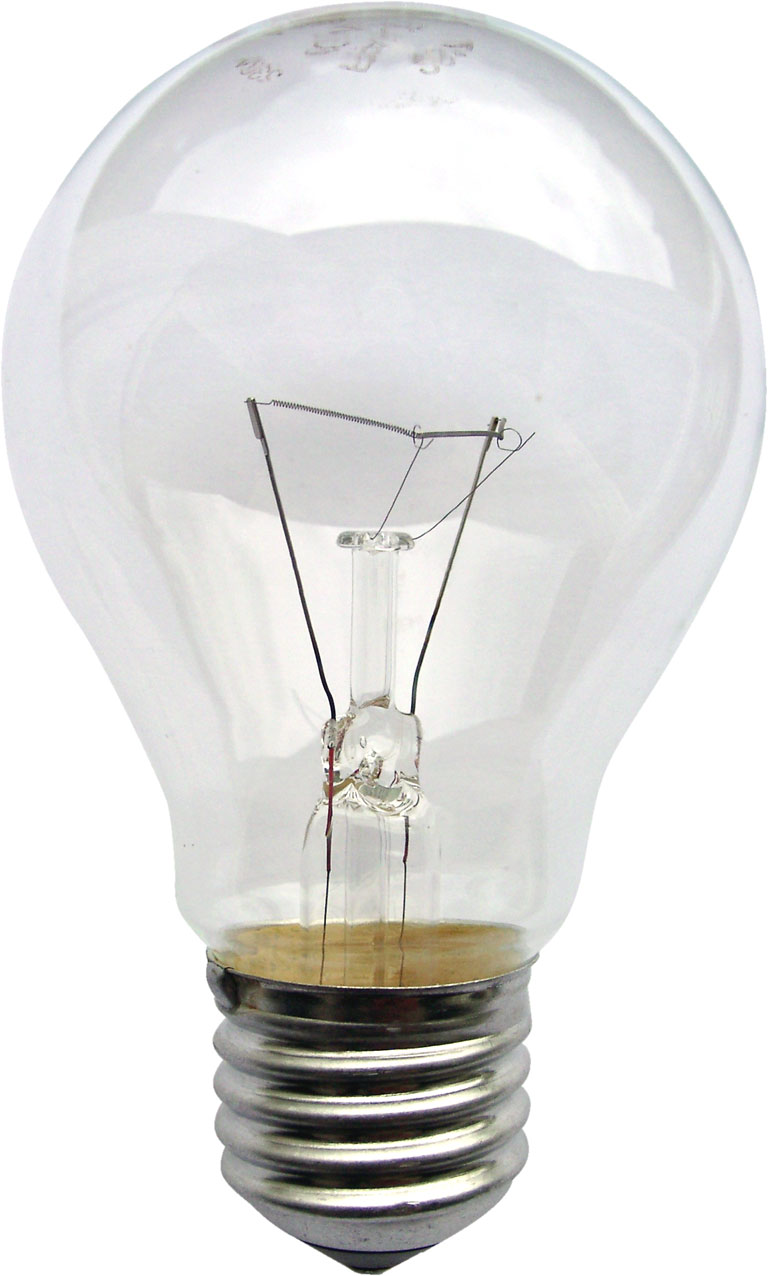
\includegraphics[width=.38\textwidth]{images/lightbulb2.png}
\end{center}

\vspace{1em}

{\tiny 
Source: Wikimedia Commons (\href{https://commons.wikimedia.org/wiki/File:06_Spiral_CFL_Bulb_2010-03-08_(white_back).jpg}{Sun Ladder}, \href{https://commons.wikimedia.org/wiki/File:Gluehlampe_01_KMJ.jpg}{KMJ}) \par }

}


\frame{

\frametitle{Example 4:\\Donations}

\begin{itemize}\itemsep1em
\item Miller and Krosnick\footnote{Miller, Krosnick, \& Lowe. N.d. ``The Impact of Policy Change Threat on Financial Contributions to Interest Groups.'' Working paper.} asked for charitable donations via cheque directly as part of a paper-and-pencil survey

\item<2-> Klar and Piston\footnote{Klar \& Piston. 2015. ``The influence of competing organisational appeals on individual donations.'' \textit{Journal of Public Policy} 35(2): 171--91. \href{http://doi.org/10.1017/S0143814X15000203}{doi:10.1017/S0143814X15000203}} offered respondents a survey incentive up-front for participation and then later offered them a chance to donate (a portion of payment) to a charity
\end{itemize}

}




\frame{

\frametitle{Example 5:\\Web Tracking Data}

\begin{enumerate}\itemsep1em
\item Active installation of a tracking app, such as YouGov Pulse\footnote{\url{https://yougov.co.uk/find-solutions/profiles/pulse/}} \footnote{Guess, AM. N.d. ``Media Choice and Moderation.'' Working paper, \url{https://dl.dropboxusercontent.com/u/663930/GuessJMP.pdf}.}

\item Post-hoc collection of web history files using something like Web Historian \footnote{\url{http://www.webhistorian.org/}}
\end{enumerate}
}



\frame<1-2>[label=other]{
\frametitle{Other Possibilities}

\begin{itemize}\itemsep1em
\item<2-> Coordination tasks
	\begin{itemize}
	\item Synchronous group tasks\footnote{Mao, Mason, Suri, Watts. 2016. ``An Experimental Study of Team Size and Performance on a Complex Task.'' \textit{PLoS ONE} 11(4): e0153048. \href{http://doi.org/10.1371/journal.pone.0153048}{doi:10.1371/journal.pone.0153048}} 
	\item Game play
	\item Simulations
	\end{itemize}
\item<3-> Offering incentives to perform future behaviour (tracked elsewhere)
\item<4-> OAuth/API integrations w/ other platforms
	\begin{itemize}
	\item Merging website usage data w/ survey data
	\item Treating website sign-up or usage as behavioural outcomes
	\item Linking with smartphone metadata
	\end{itemize}
\end{itemize}
}

\frame{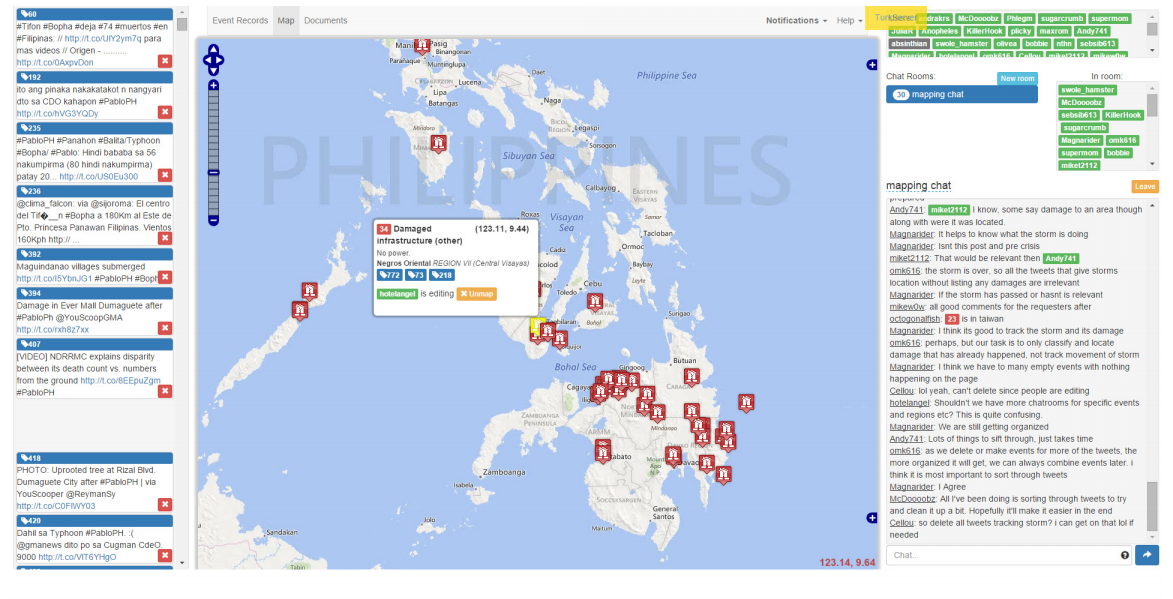
\includegraphics[width=\textwidth]{images/mao.png}}


\againframe<2->{other}


\frame{}

\frame{

\large 

\begin{center}
With a partner, brainstorm how one or more these behavioural measures might be applied to a survey data collection relevant to your own work or your organisation.
\end{center}

}


\frame{}



\section{Conclusion}
\frame{\tableofcontents[currentsection]}



\frame{

\frametitle{Some principles for survey measures of behaviour}

\begin{enumerate}\itemsep1em
\item<2-> Know why you are collecting a behavioural measure!
\item<3-> Know whether you are studying a past, present, or future behaviour.
\item<4-> Be creative! Recognise possibilities and limitations of any given survey mode.
\item<5-> Validate, validate, validate!
\end{enumerate}

}

\frame{}

\frame{
\frametitle{To Sum Up\dots}

\begin{itemize}\itemsep1em
\item Surveys are well-designed to measure current characteristics, beliefs, and attitudes
\item Self-report measures of behaviour have many problems
\item Surveys can incorporate direct measures of respondent behaviour
\item We're still experimenting, so more research is needed on validity of such measures
\end{itemize}
}


\frame{


\large
\begin{center}

\textbf{Thanks!}\\

\vspace{1em}

I will be around for questions.\\ 
Don't hesitate to be in touch later on:\\

\vspace{1em}

Email: \href{mailto:t.leeper@lse.ac.uk}{t.leeper@lse.ac.uk}\\
Twitter: \href{https://twitter.com/thosjleeper}{@thosjleeper}

\end{center}

}




\appendix
\frame{}



\section{References}



\end{document}
